	\documentclass{beamer}
\usepackage[utf8]{inputenc}

\usetheme{Madrid}

%% ADDITIONAL NICOLÁS
\usepackage{ragged2e}
\usepackage{amssymb}
\usepackage{subcaption}

\usefonttheme{serif}
\definecolor{UBCblue}{rgb}{0.01569, 0.11765, 0.25882} % PSU Blue
\usecolortheme[named=UBCblue]{structure}

%% ADDITIONAL NICOLÁS




%------------------------------------------------------------
%This block of code defines the information to appear in the
%Title page
\title[Weekly Reports] %optional
{PhD in Energy and Mineral Engineering at PSU}

\subtitle{Nicolás's Research - Reports}

\author[Nicolás Bueno] % (optional)
{Nicolás Bueno\inst{1} \and Advisor: Dr. Ayala\inst{1}}

\institute[EME] % (optional)
{
	\inst{1}%
	Department of Energy and Mineral Engineering\\
	Penn State University\\
	
\includegraphics[height=1cm]{pics/PSU_EMS.png}
}

\date[Spring 2022] % (optional)
{}

%\logo{
\includegraphics[height=1cm]{pics/PSU_EMS.png}}

%End of title page configuration block
%------------------------------------------------------------



%------------------------------------------------------------
%The next block of commands puts the table of contents at the 
%beginning of each section and highlights the current section:

\AtBeginSection[]
{
	\begin{frame}
		\frametitle{Table of Contents}
		\tableofcontents[currentsection]
	\end{frame}
}
%------------------------------------------------------------


\begin{document}
	
	%The next statement creates the title page.
	\frame{\titlepage}
	
	%---------------------------------------------------------
	%This block of code is for the table of contents after
	%the title page
	\begin{frame}
		\frametitle{Table of Contents}
		\tableofcontents
	\end{frame}
	%---------------------------------------------------------
	
	\justifying
	\section{Spring 2022}
	
	\subsection{Report Jan 24 - 2022}
	\label{}
	\justifying
	\begin{frame}
		\textbf{Report Jan 24 - 2022}\\~\\
		Main discussion points:
		\begin{itemize}
			\item Cheng's paper
			\item LBM Code state
			\item Short-term Medium-term objectives
		\end{itemize}
	\end{frame}
	
	\begin{frame}{Cheng's paper}
		Bulk equation for the Shan-Chen force:
		\begin{equation*}
		\mathbf{F} = -G \psi(x) \sum_i \omega_i \psi(x+\mathbf{c}_i \delta t) \mathbf{c}_i \, \, \, \, \, \psi := \sqrt{\frac{2(P^{\text{\tiny EoS}}-c_s^2\rho)}{G \delta t c_s^2}}
		\end{equation*}
		\begin{itemize}
			\item MRT model
			\item Multi-component partially miscible
		\end{itemize}
	\end{frame}
	
	\begin{frame}{LBM state}
		This I advanced before last state:
		\begin{itemize}
			\item Tried the binary printing (unsuccessful)
			\item Run the single component multi-phase model (successful)
			\item Equation to count the number of molecules in a lattice. 
			\item Short-term mid-term objectives
		\end{itemize}
	\end{frame}

	\begin{frame}{van der Waals validation}
		\begin{figure}
			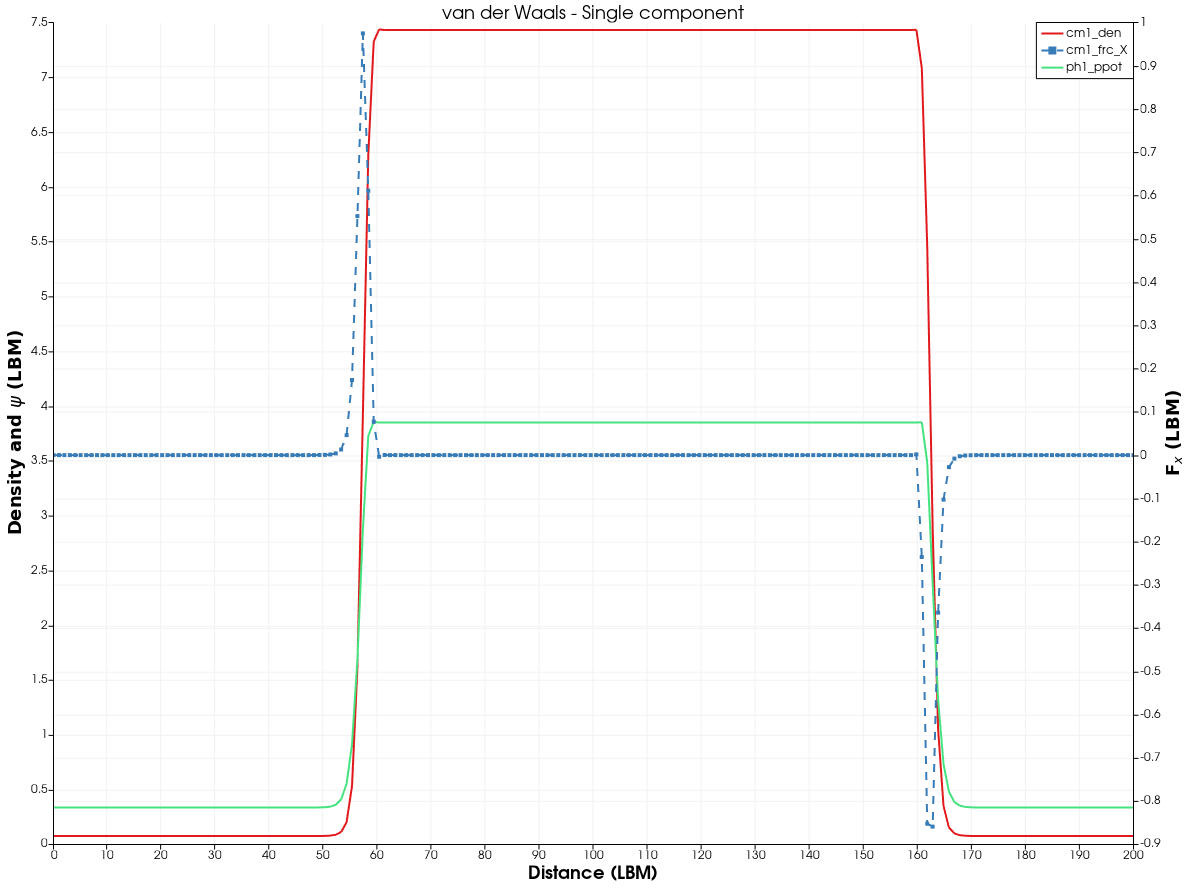
\includegraphics[scale=0.2]{pics/vdwValidation.png}
		\end{figure}
	\end{frame}

	\begin{frame}{Peng Robinson validation}
		\begin{columns}
			\column{0.4\textwidth}
			\begin{figure}
				\centering
				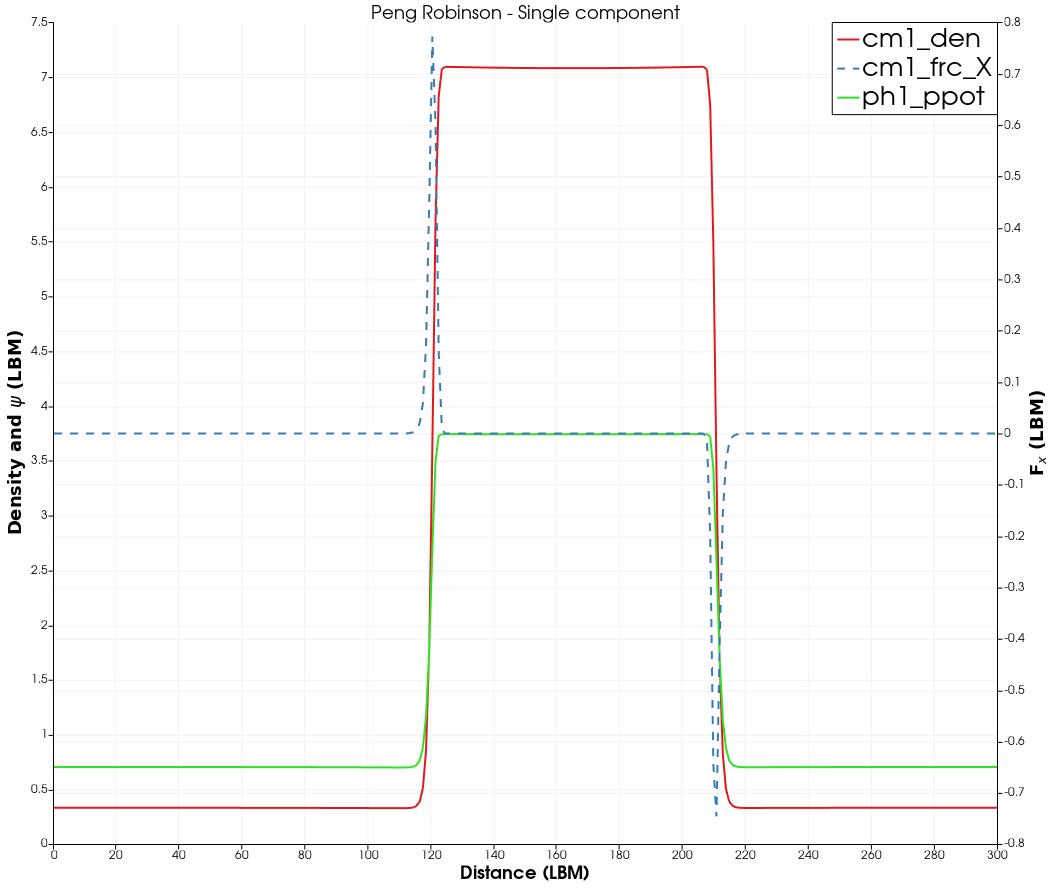
\includegraphics[scale=0.12]{pics/prValidation.png}
				\caption{}   
			\end{figure}
			\column{0.4\textwidth}
			\begin{figure}
				\centering
				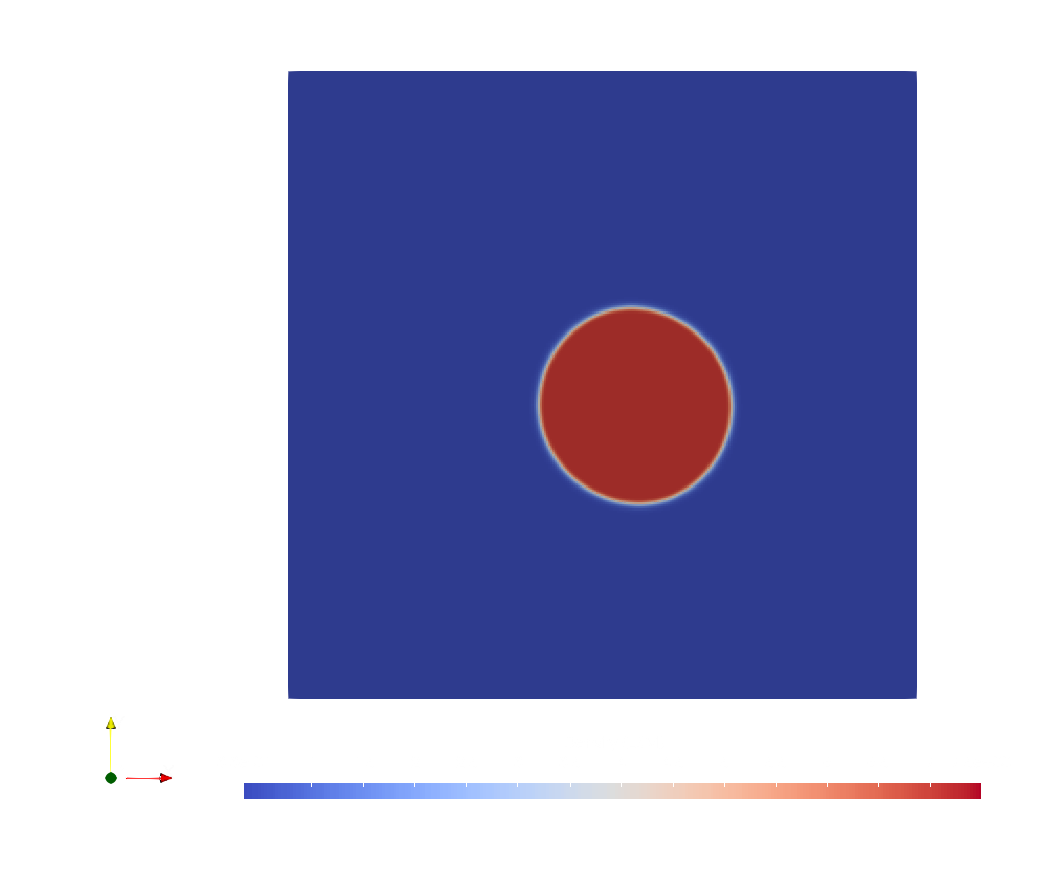
\includegraphics[scale=0.15]{pics/prValidation2.png}
			\end{figure}
		\end{columns}
	\end{frame}

	\begin{frame}{Where I am going?}
		I was rediscovering the concept of $\psi$ that now belongs to the bulk (phase) entity. In Kruger's book is assigned to each component, so each components computes its own SC force. Other forces split according to $\rho_i$.\\
		Two components structure is ready to start building the 2-component case that Cheng uses for validation. 
	\end{frame}
	\begin{frame}{Actions}
		\begin{itemize}
			\item Dry-run of research proposal for qualifying exam.Deep dive into literature looking for problems in current problems and interesting applications (reactions-solute transport-energy-multiphase).
			\item LBM tutorials is the next short-term project
			\item Finish my own code to run the Cheng's cases in our simulator. 
			\item Long-term: evaluate the Kruger's perspective of calculating SC per component.
		\end{itemize}
	\end{frame}
	
	%---------------------------------------------------------
	%---------------------------------------------------------
	\subsection{Report Jan 31 - 2022}
	\label{}
	\justifying
	\begin{frame}
		\textbf{Report Jan 31 - 2022}\\~\\
		\begin{itemize}
			\item Code and Cheng's paper
			\item SPH for EME 521
			\item Time demand
			\item Others
			\begin{itemize}
				\item Dr. Mehmani meetings (I'll start slow). 
				\item Summer 2022
				\item Almost null offer research-related. Italian courses.
				\item STAP (Summer Tuition Assistance Program)
				\item Penn State Vita (Taxes)
				\item 2022 Fuel Science Graduate Awards
				\item Own website
			\end{itemize}
			\item Lost.
		\end{itemize}
	\end{frame}
	
	\begin{frame}{Code}
		Multiphase validations: van der Waals (flat interface, droplet), Peng-Robinson (making use of velocity redefinition and $\beta$ parameter).\\
		Cheng redefined the velocity for the Guo's scheme as:
		
		\begin{equation}
			\mathbf{u}^{mod} = \mathbf{u} + \frac{\beta \mathbf{F}}{(\tau - 0.5)\psi^2}
		\end{equation}
		
		The other velocity definitions remain. Without this term, the PR case diverges. Also $G$ affects stability.
		
	\end{frame}
	
	\begin{frame}{Code - Peng Robinson validation}
		\begin{columns}
			\column{0.4\textwidth}
			\begin{figure}
				\centering
				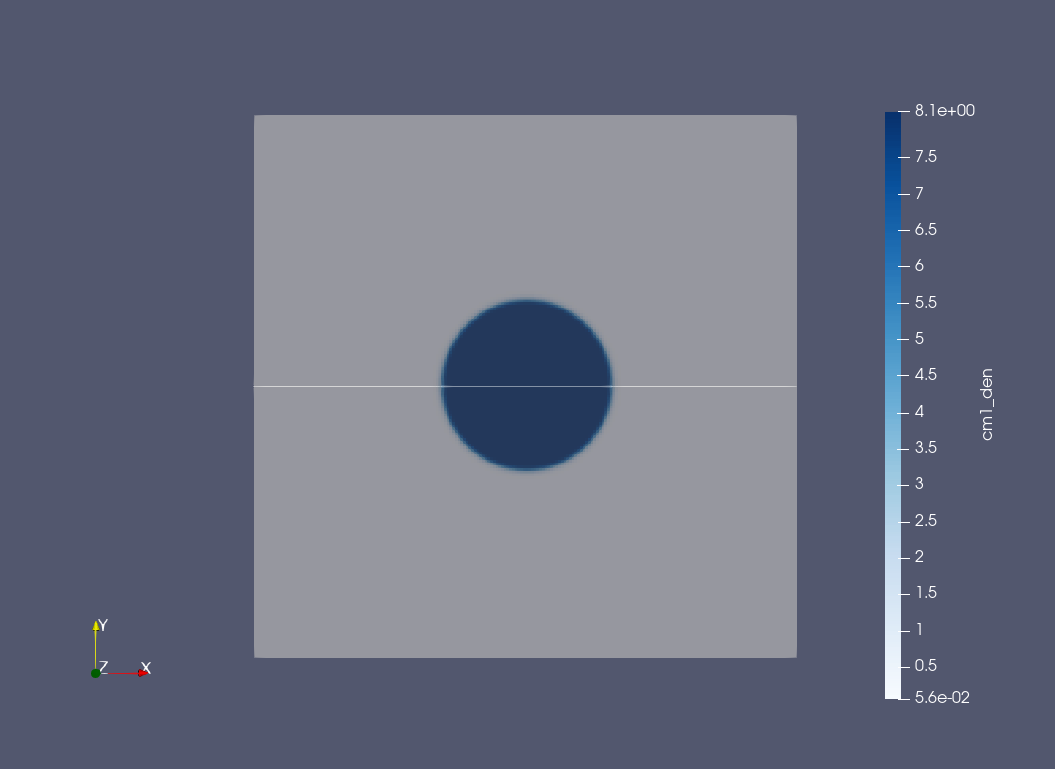
\includegraphics[scale=0.12]{pics/prDroplet1C.png}
				\caption{}   
			\end{figure}
			\column{0.4\textwidth}
			\begin{figure}
				\centering
				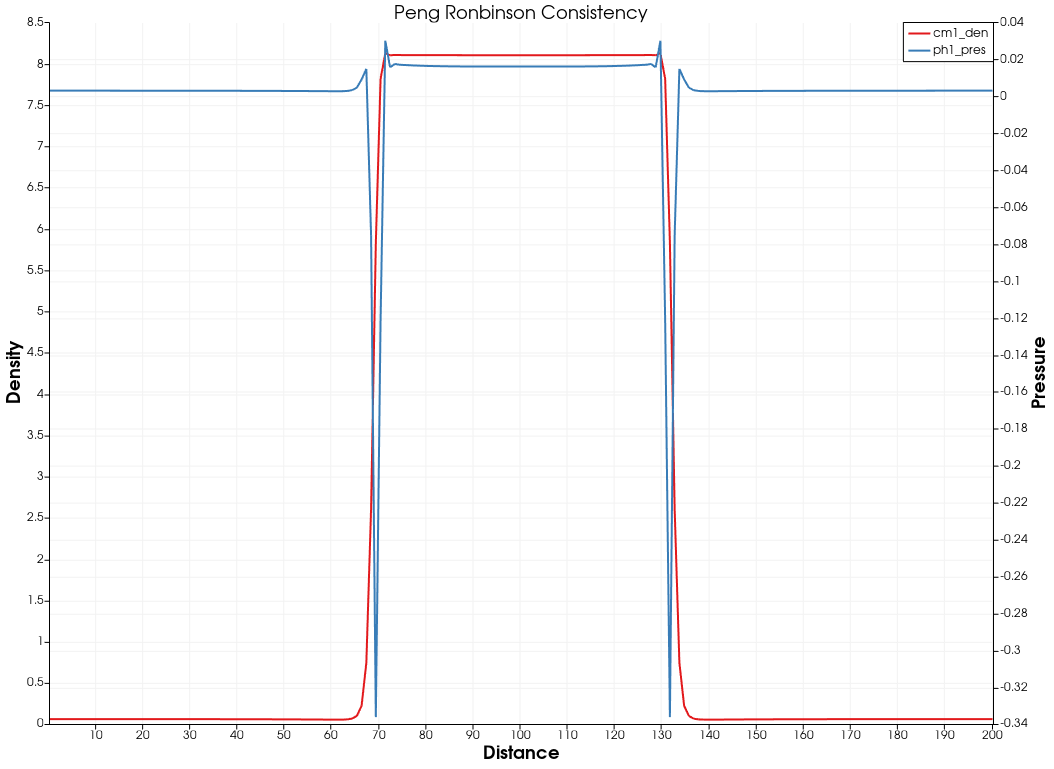
\includegraphics[scale=0.15]{pics/prDroplet1C_2.png}
			\end{figure}
		\end{columns}
	\end{frame}
	
	\begin{frame}{Code - New features}
		\begin{itemize}
			\item Now we can have $N_F$ forces of different nature. All are grouped and discretized in the velocity space together.
			\item We have now a new force to compute $\psi^i$ and thus calculate a force per component.
			\item Each component relaxes with its own $\tau^i$, allowing different viscosities.
			\item Reading density/pressure fields for every component, and a common velocity field.
		\end{itemize}
		Current problems:
		\begin{itemize}
			\item Force only working for periodic BC.
			\item Still not implemented the force fluid/solid
			\item Instability (due to BGK)
		\end{itemize}
		 
	\end{frame}
	
	\begin{frame}{Code}
		\begin{itemize}
		\item Can the pressure of the gas be higher than the liquid? What if we initialize a bubble instead of a droplet?
		\item Validate Young-Laplace?
		\item I am now setting a 2C 2P problem to validate the code. I can try both, immiscible and miscible, as both implementations are there and the only change is the $\psi$ definition.
		\item Injecting A into a system full of B. How does it look like?
		\item What 1C complex systems can we simulate? Water hammer effect?
		\end{itemize}
		Ready for meeting with Pr. Orlando for program. language discussions, questions about implementations, and possible feedback (I need the time to compile the material).\\~\\
		
		PBM: RR procedure. I'll program the minimization algorithm, but try to implement Eigen, a library to solve $\mathbf{A \cdot x} = \mathbf{b}$.
	\end{frame}
	
	\begin{frame}{Research}
		I definitely want to use my research for applying the LBM to a particular field. In contrast, my Master's Thesis was only computational, with validations, but did not include any experimental/real data of any type. Questions I have:
		\begin{itemize}
			\item Bubbles, coalescence, and their viscosity effect
			\item CO$_2$ plume generation.
			\item Interaction between fluids and rock (swelling, mineralization, adsorption)
			\item Rock deformation? Does imply FEM? Too complicated? 
			\item Questions about $\sigma$ in 3-P systems. I don't know? Nobody knows? Film drainage. Oil spills. Receding / advancing $\theta$ 
			\item Can we derive a $k_r$ label-blind with hysteresis, based on 3P simulations?
		\end{itemize}
		
	\end{frame}

	\begin{frame}{Actions}
		\begin{itemize}
			\item Yes, start learning SPH. 
			\item Look for internships in companies and research labs in the US. In Summer, if nothing appears, we will focus on research. Do not lose contacts and willingness to participate in new things.
			\item Apply to Fuel Award and Nico SPE Awards
			\item Go for MRT. Write equations. Pr. Orlando presentation. Think in 2C cases that validates our understanding. 2 non interacting components (miscible). Then partially miscible. 
			\item Bubbles as an interesting topic to work with in LBM. There may be other options.
		\end{itemize}
	\end{frame}
	%---------------------------------------------------------
	%---------------------------------------------------------
	
	\begin{frame}{Discussion}
		Discussion...
	\end{frame}
	
	%---------------------------------------------------------
	%---------------------------------------------------------
	
	\subsection{Report Feb 7 - 2022}
	\label{}
	\justifying
	\begin{frame}
		\textbf{Report Feb 7 - 2022}\\~\\
		\begin{itemize}
			\item Cheng's coding error in modified velocity.
			\item MRT implementation. Facts and difficulties:
			\begin{itemize}
				\item Vectorized implementation. Still have problems with $\mathbf{m}^{\text{eq}}$. Works only in manual computing.
				\item More validation cases. I only picked one.
				\item Recent result: yesterday.
			\end{itemize}
			\item Peng Robinson inconsistency: I have to revisit the PR results with BGK. I thing it may be converging to densities slightly away from equilibrium.
			\item Dr. Mehmani suggestions.
			
		\end{itemize}
	\end{frame}
	

	\begin{frame}{MRT Validation}
		\begin{figure}
			\centering
			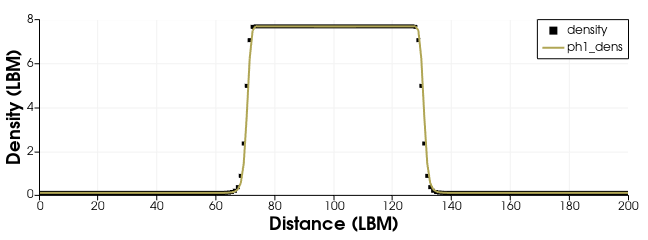
\includegraphics[scale=0.4]{pics/MRTValDen.png}
		\end{figure}
		\begin{figure}
			\centering
			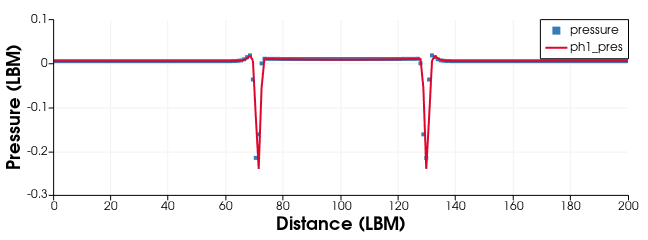
\includegraphics[scale=0.4]{pics/MRTValPres.png}
		\end{figure}
	
	\end{frame}
	\begin{frame}{Actions}
		\begin{itemize}
			\item Prepare meeting with Cheng: velocity modification, and MRT parameters. Source of validation.
			\item Trace a path for validation: Oscillating droplet, tube oscillation. 
			\item Reading CO$_2$ with oil trapping and water different mechanisms and modeling.
			\item Share code.
			
		\end{itemize}
	\end{frame}
	
	
	%---------------------------------------------------------
	%---------------------------------------------------------
	
	\subsection{Report Feb 14 - 2022}
	\label{}
	\justifying
	\begin{frame}
		\textbf{Report Feb 14 - 2022}\\~\\
		\begin{itemize}
			
			\item BGK and MRT validations
			\begin{itemize}
				\item Several cases tested: see the LBM private document
				\item How to set fluid viscosity with MRT?
				\item I had to change Cheng's diffuse width.
			\end{itemize}
			
			\item Dr. Mehmani suggestions.
			\item Questions
			\begin{itemize}
				\item Point-distributed parameter and point-centered (?) parameter
				\item Fluid in tension LBM?
				\item Motivation. Self-propulsion, drop collision, microemulsions: \href{https://www.youtube.com/watch?v=arpGntfrg4s}{link to Youtube}
			\end{itemize}
			
		\end{itemize}
	\end{frame}

	\begin{frame}{BGK Validation - Cheng's code}
		\begin{figure}
			\centering
			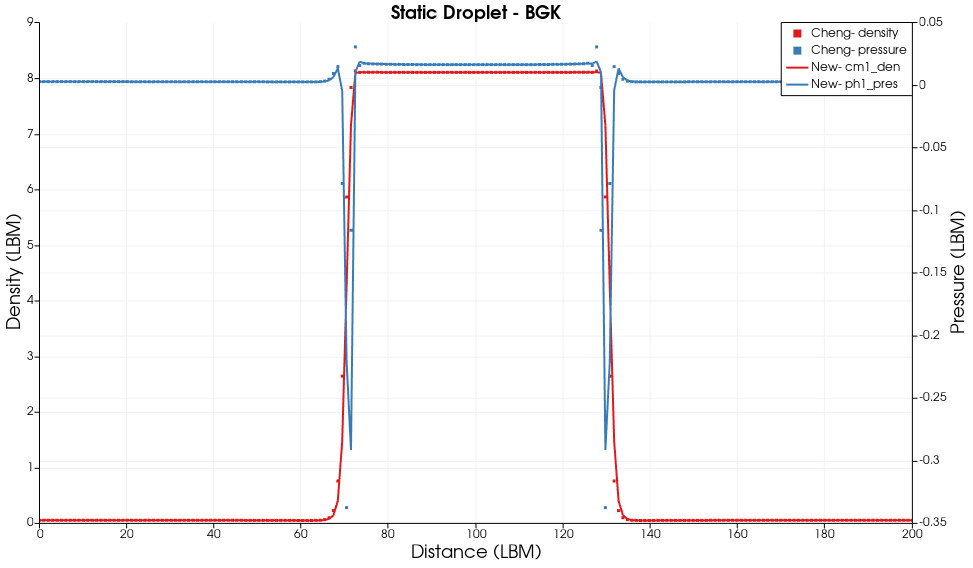
\includegraphics[scale=0.3]{pics/BGK_StaticDroplet.png}
		\end{figure}
	\end{frame}
	\begin{frame}{BGK Validation - Cheng's code}
		\begin{figure}
			\centering
			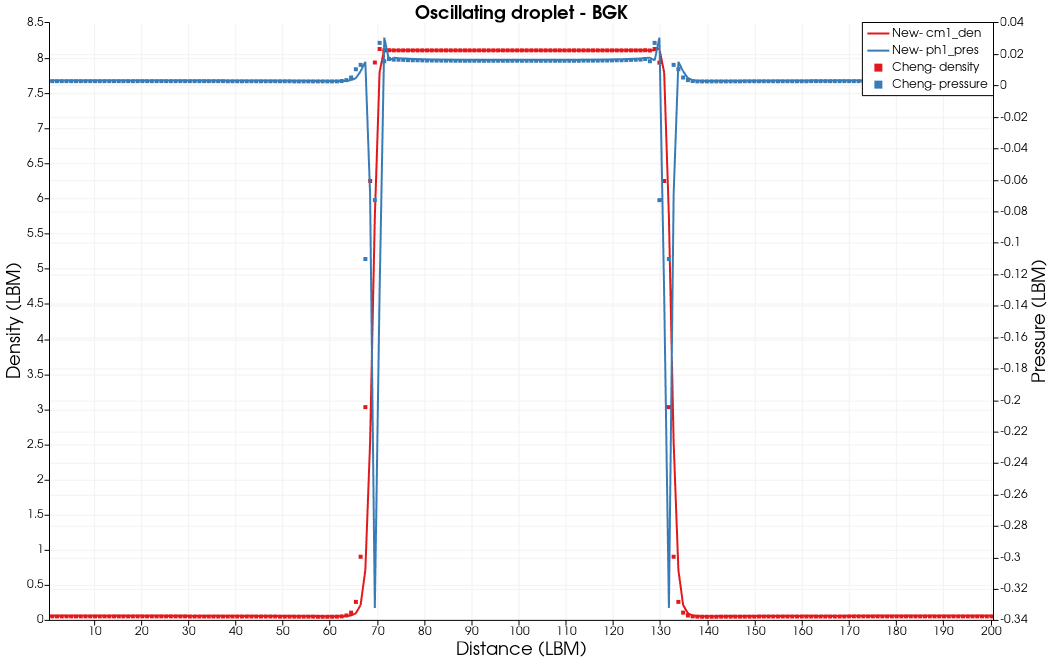
\includegraphics[scale=0.3]{pics/BGK_OscDroplet_PRHO.png}
		\end{figure}
	\end{frame}
	\begin{frame}{BGK Validation - Cheng's code}
		\begin{figure}
			\centering
			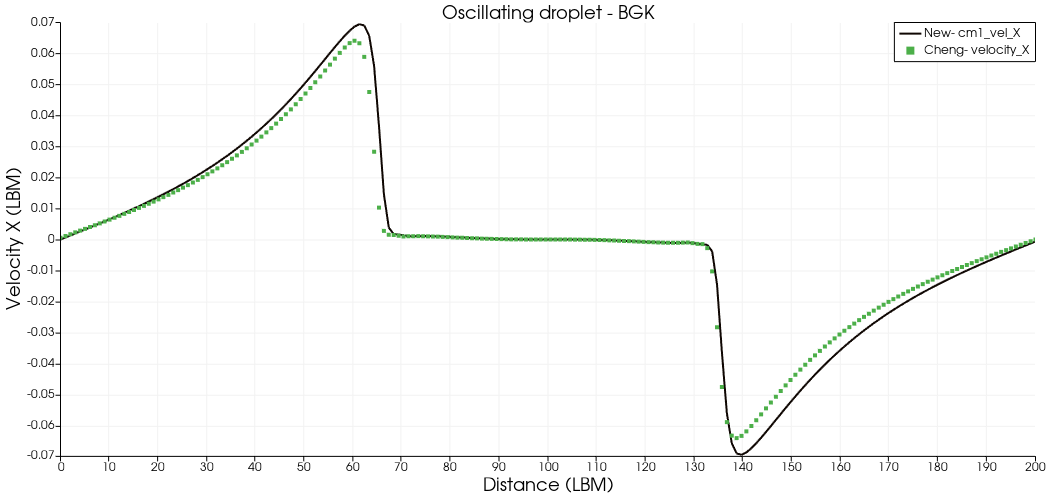
\includegraphics[scale=0.3]{pics/BGK_OscDroplet_VelProf.png}
		\end{figure}
	\end{frame}
	\begin{frame}{BGK Validation - Cheng's code}
		\begin{figure}
			\centering
			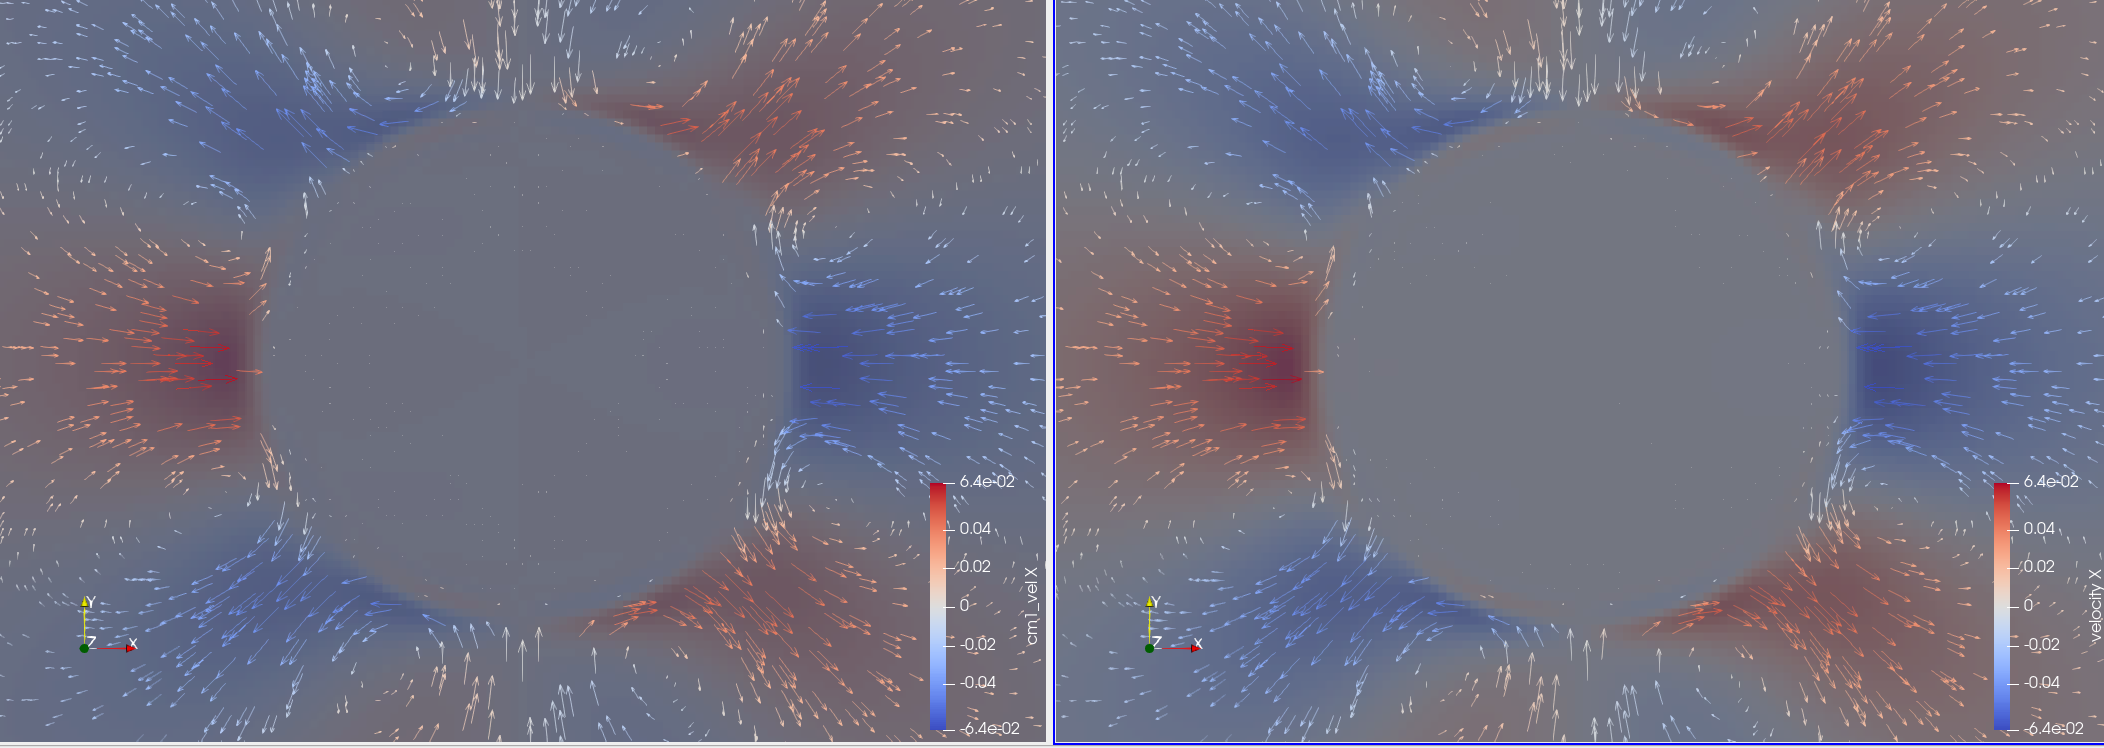
\includegraphics[scale=0.14]{pics/BGK_VelFieldComparison.png}
		\end{figure}
	\end{frame}
	\begin{frame}{BGK Validation - Cheng's code}
		\begin{figure}
			\centering
			\includegraphics[scale=0.14]{pics/OScDroplet_BGK_Axis.png}
		\end{figure}
	\end{frame}
	
	
	\begin{frame}{MRT Validation - Cheng's code}
		\begin{figure}
			\centering
			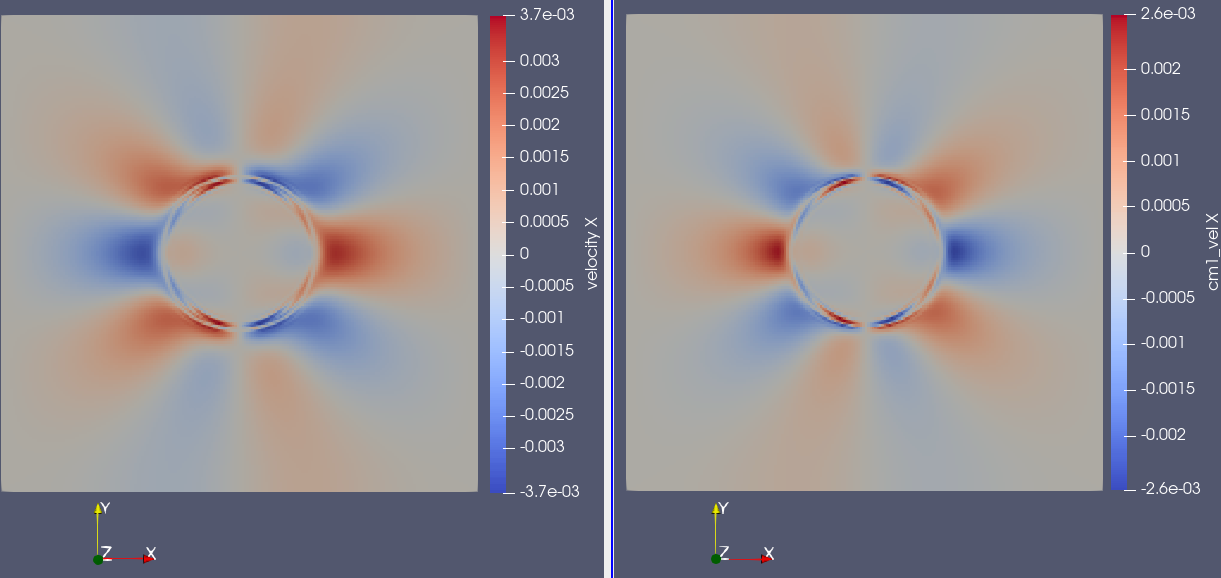
\includegraphics[scale=0.25]{pics/MRT_StaticDroplet_VelField.png}
		\end{figure}
	\end{frame}
	\begin{frame}{MRT Validation - Cheng's code}
		Attached video.
		\begin{figure}
			\centering
			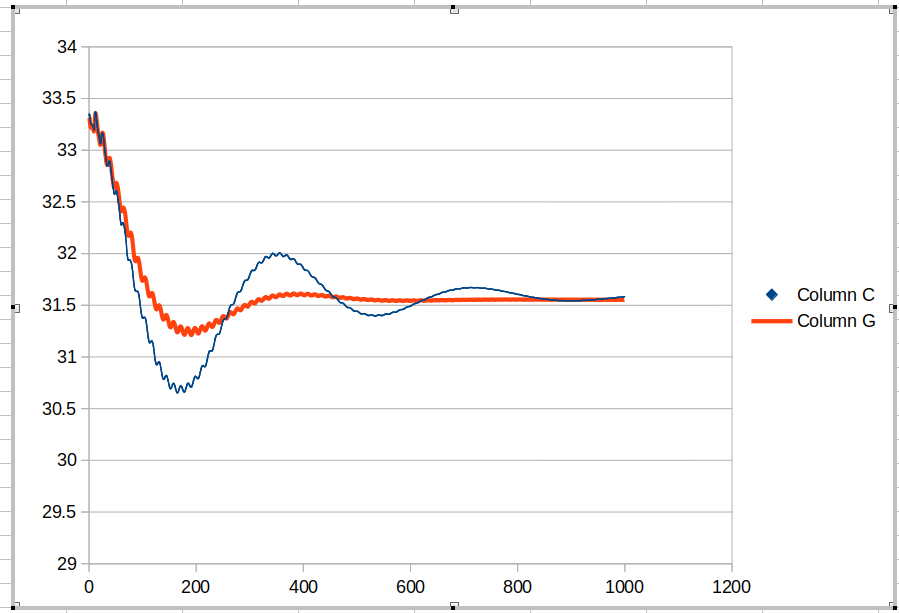
\includegraphics[scale=0.25]{pics/MRT_oscillatingAxis.png}
		\end{figure}
	\end{frame}
	
	\begin{frame}{For analytical solutions}
		\begin{itemize}
			\item How to convert a single component droplet surrounded by its vapor, to a droplet surrounded by empty space? Is the frequency of the oscillation the same in both cases.
			
			\item Analytical solutions and reported cases:
			\begin{itemize}
				\item Oscillating droplet
				\item Rising bubble (very interesting!)
				\item Square drop as IC
				\item Rayleigh-Taylor instability (heavy fluid supported against gravity)
				\item Induced translation by Marangoni-effect (variable $\sigma$ field)
				\item Bubble break-up due to variable $\sigma field$
			\end{itemize}
		\end{itemize}
	\end{frame}

	\begin{frame}{Actions}
		\begin{itemize}
			\item Keep preparing Cheng's meeting
			\item Go back to BGK and compare oscillations
			\item Find differences with MRT for oscillating droplet
			\item Start reading LAMP reference and Cheng's reports to compare against analytical solution
			\item Go for the 2 components case
		\end{itemize}
	\end{frame}
	
	
	%---------------------------------------------------------
	%---------------------------------------------------------
	
	
	\subsection{Report Feb 21 - 2022}
	\label{}
	\justifying
	\begin{frame}
		\textbf{Report Feb 21 - 2022}\\~\\
		\begin{itemize}
			\item BGK and MRT validations
			\item Viscosity per phase-per component
			\item Rising droplet (video)
			\item Marangoni flow (papers based on Phase-Field and Free energy)
			\item Questions
			\begin{itemize}
				\item Point-distributed parameter and point-centered (?) parameter
				\item Fluid in tension LBM?
				\item Motivation. Self-propulsion, drop collision, microemulsions: \href{https://www.youtube.com/watch?v=arpGntfrg4s}{link to Youtube}
			\end{itemize}
			\item What to present in next meeting?
		\end{itemize}
	\end{frame}

	\begin{frame}{Oscillating droplet}
		\begin{figure}[h]
			\centering
			\begin{subfigure}{.5\textwidth}
				\centering
				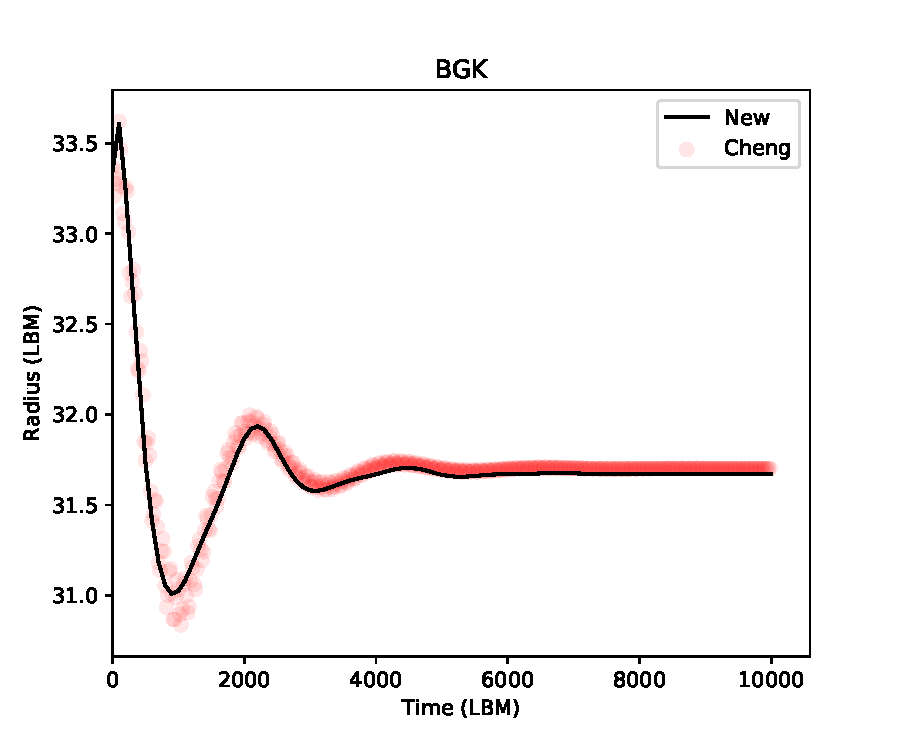
\includegraphics[width=.9\linewidth]{pics/BGKOsc.pdf}
				\caption{BGK}
				\label{fig:sub1}
			\end{subfigure}%
			\begin{subfigure}{.5\textwidth}
				\centering
				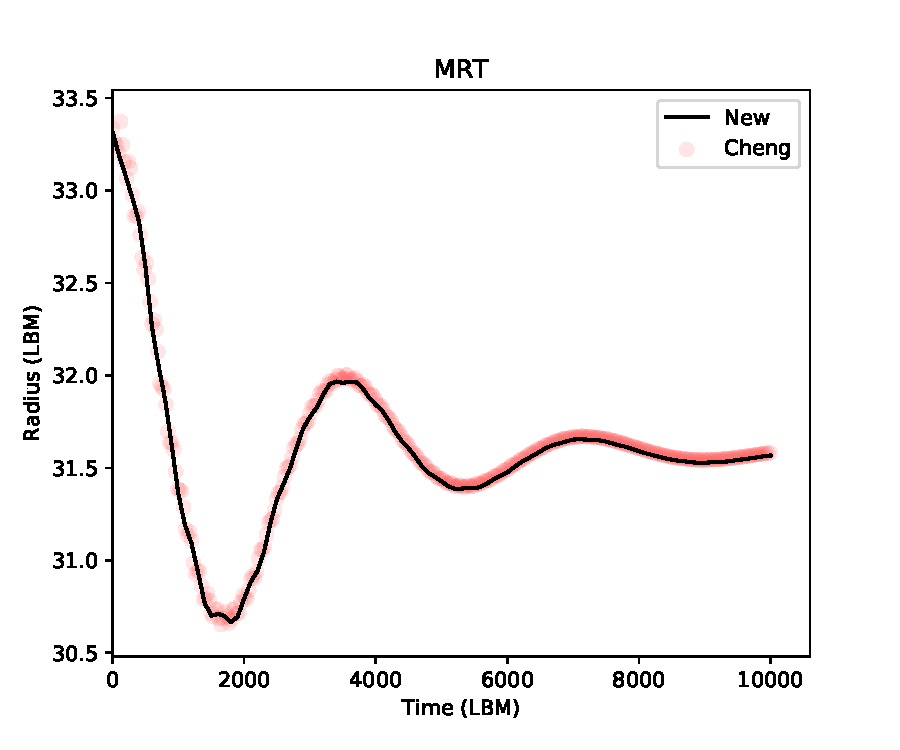
\includegraphics[width=.9\linewidth]{pics/MRTOsc.pdf}
				\caption{MRT}
				\label{fig:sub2}
			\end{subfigure}
			\caption{Oscillation droplet case. Viscosities are different in each case.}
			\label{fig:osci}
		\end{figure}
	\end{frame}

	\begin{frame}{Thursday meeting}
		\begin{itemize}
			\item Motivation of new code
			\item Current validations
			\item Current status
			\item Questions about: boundary conditions, global density increase, dynamic validations:
			\begin{itemize}
				\item Oscillating droplet (ready). For which conditions, an analytical solution exists? Droplet in void space?
				\item Rayleigh-Taylor instability (oscillating capillary tube)
				\item Rotating droplet (any analytical solution)
			\end{itemize}
		\end{itemize}
	\end{frame}
	
	
	
	\begin{frame}{Actions}

	\end{frame}

	%---------------------------------------------------------
	%---------------------------------------------------------

	\subsection{Weekly meeting - LBM - Feb 24 - 2022}
	\label{}
	\justifying
	\begin{frame}{Weekly meeting - LBM}
		\textbf{Feb 24 - 2022}\\~\\
		\begin{itemize}
			\item LBM Code - New version (motivation, state, and validation)
			
			\item Questions about the LBM formulation
		
			\item Paper (Dynamic validations)
		\end{itemize}
	\end{frame}
	
	\begin{frame}{LBM Code}
		
		Motivation: 
		\begin{itemize}
			\item 3D version for arbitrary domains, forces, and boundary conditions
			\item Future parallelization
			\item Coupling with other transport equations
		\end{itemize}
	
		~\\\textbf{General description}: Fortran 90, Object Oriented, LBM code for multi-component ($N_c$) mixtures. Output in VTK format. Main classes:
		\begin{itemize}
			\item Components - Phase - Mixture - Equation of state
			\item LBM Functions (Parameters - Coll. Operators) 
			\item Domain - Global Properties
			\item Forces - Boundaries
		\end{itemize}
		Desired simulation setup is given through input files (parameters, domain, initial conditions).
	\end{frame}
	
	\begin{frame}{Validations}
		
		The main validation sources are: analytical solutions, Cheng's codes, qualitative physics understanding.\\~\\

		
		\begin{columns}[T]
			
			\column{0.5\textwidth}
			Single phase:
			\begin{itemize}
				\item Channel flow ($\mathbf{F}$ \& $\nabla p$-driven)
				\item Couette flow (plates)
				\item Cylinder (turbulent)
				\item Cavity flow
				\item Porous medium
			\end{itemize}
			
			\column{0.5\textwidth}
			Multiphase:
			\begin{itemize}
				\item Static droplet
				\item Oscillation droplet
				\item Falling droplet
			\end{itemize}
		\end{columns}
	\end{frame}

	\begin{frame}{Single phase validations (quantitative)}
		\begin{figure}[h]
			\centering
			\begin{subfigure}{.5\textwidth}
				\centering
				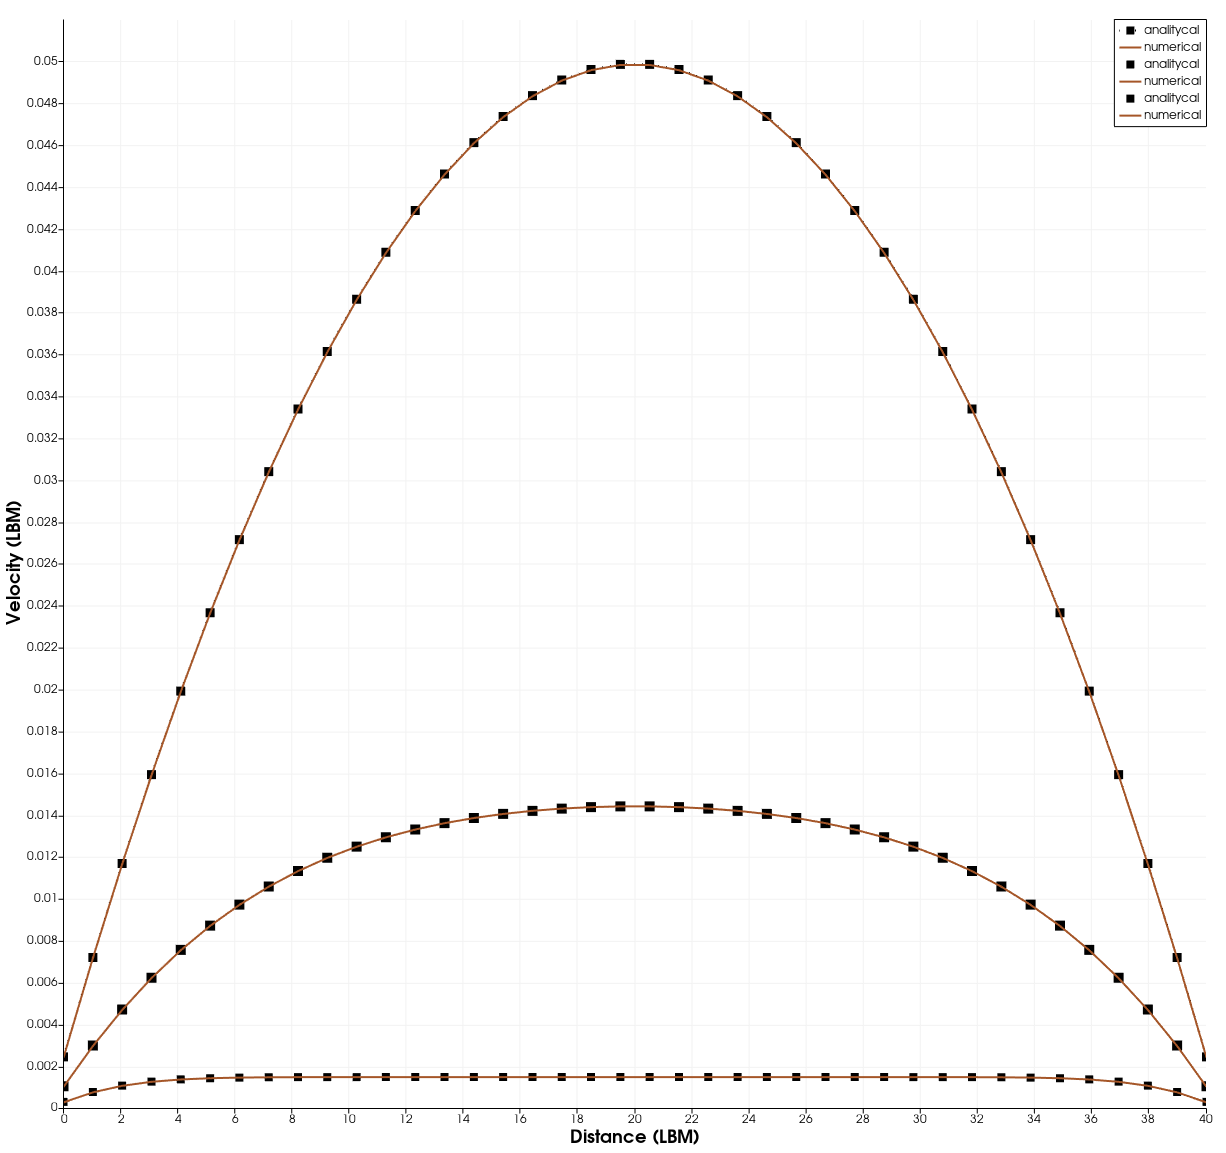
\includegraphics[width=.9\linewidth]{pics/channelForceDrivenValidation.png}
				\caption{$\mathbf{F}$-driven channel flow}
				\label{fig:sub1}
			\end{subfigure}%
			\begin{subfigure}{.5\textwidth}
				\centering
				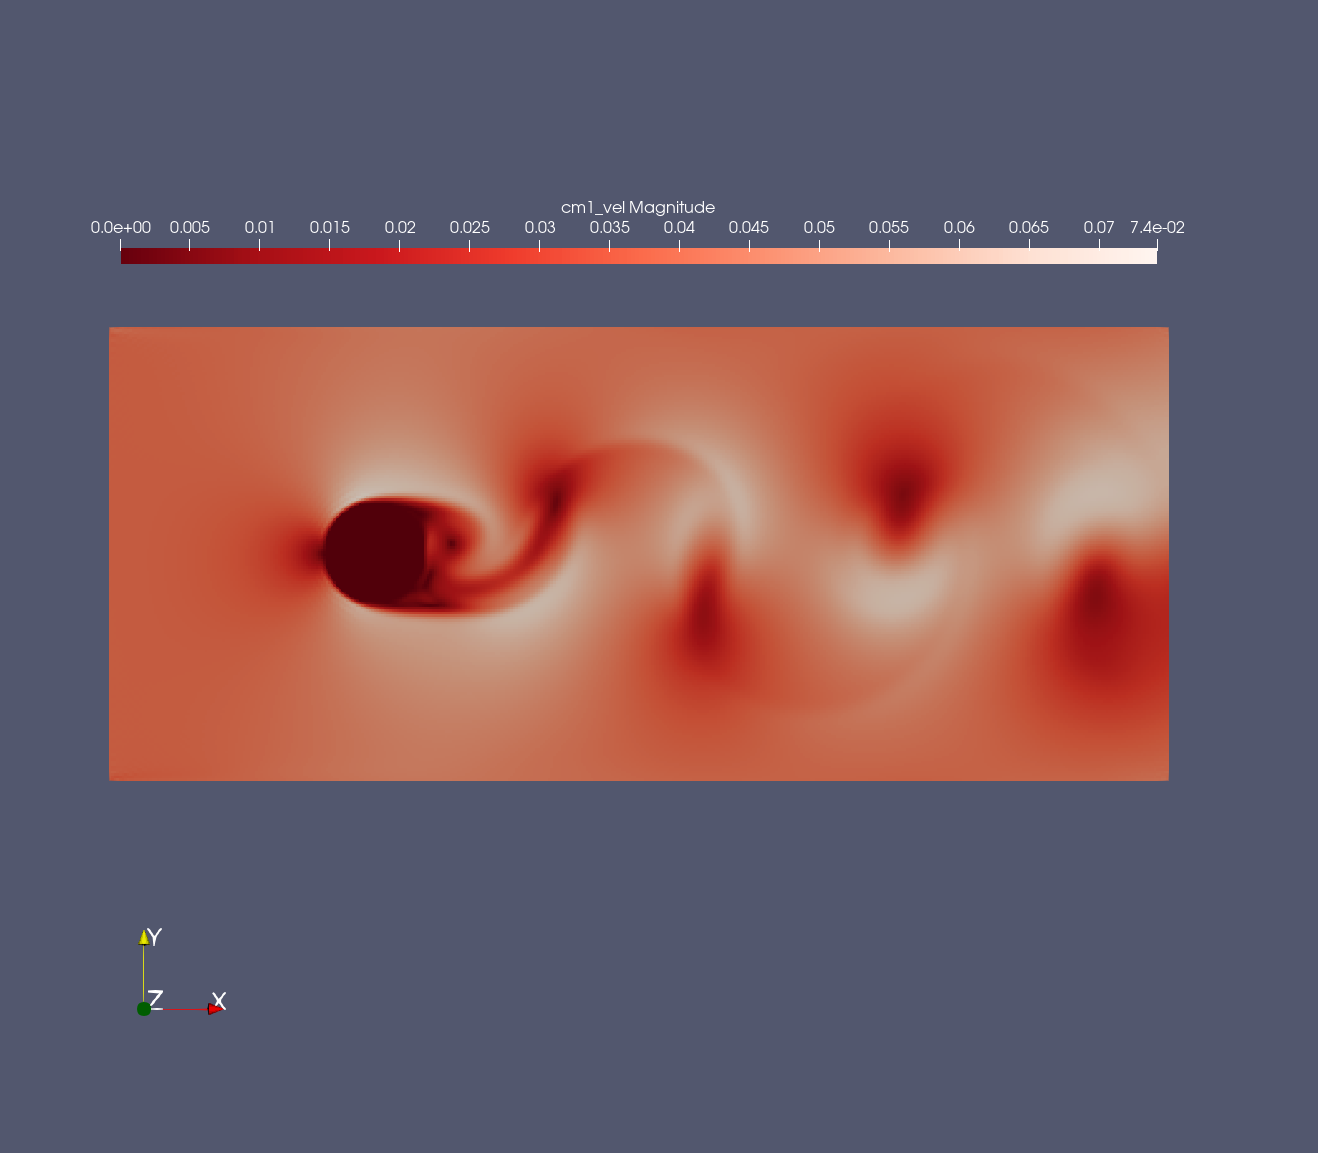
\includegraphics[width=.9\linewidth]{pics/cylinderTurbulent.png}
				\caption{Turbulent flow around cylinder}
				\label{fig:sub2}
			\end{subfigure}
			\caption{Results with direct source for quantitative comparisons.}
			\label{fig:osci}
		\end{figure}
	\end{frame}
	
	\begin{frame}{Single phase validations (qualitative)}
		\begin{figure}[h]
			\centering
			\begin{subfigure}{.5\textwidth}
				\centering
				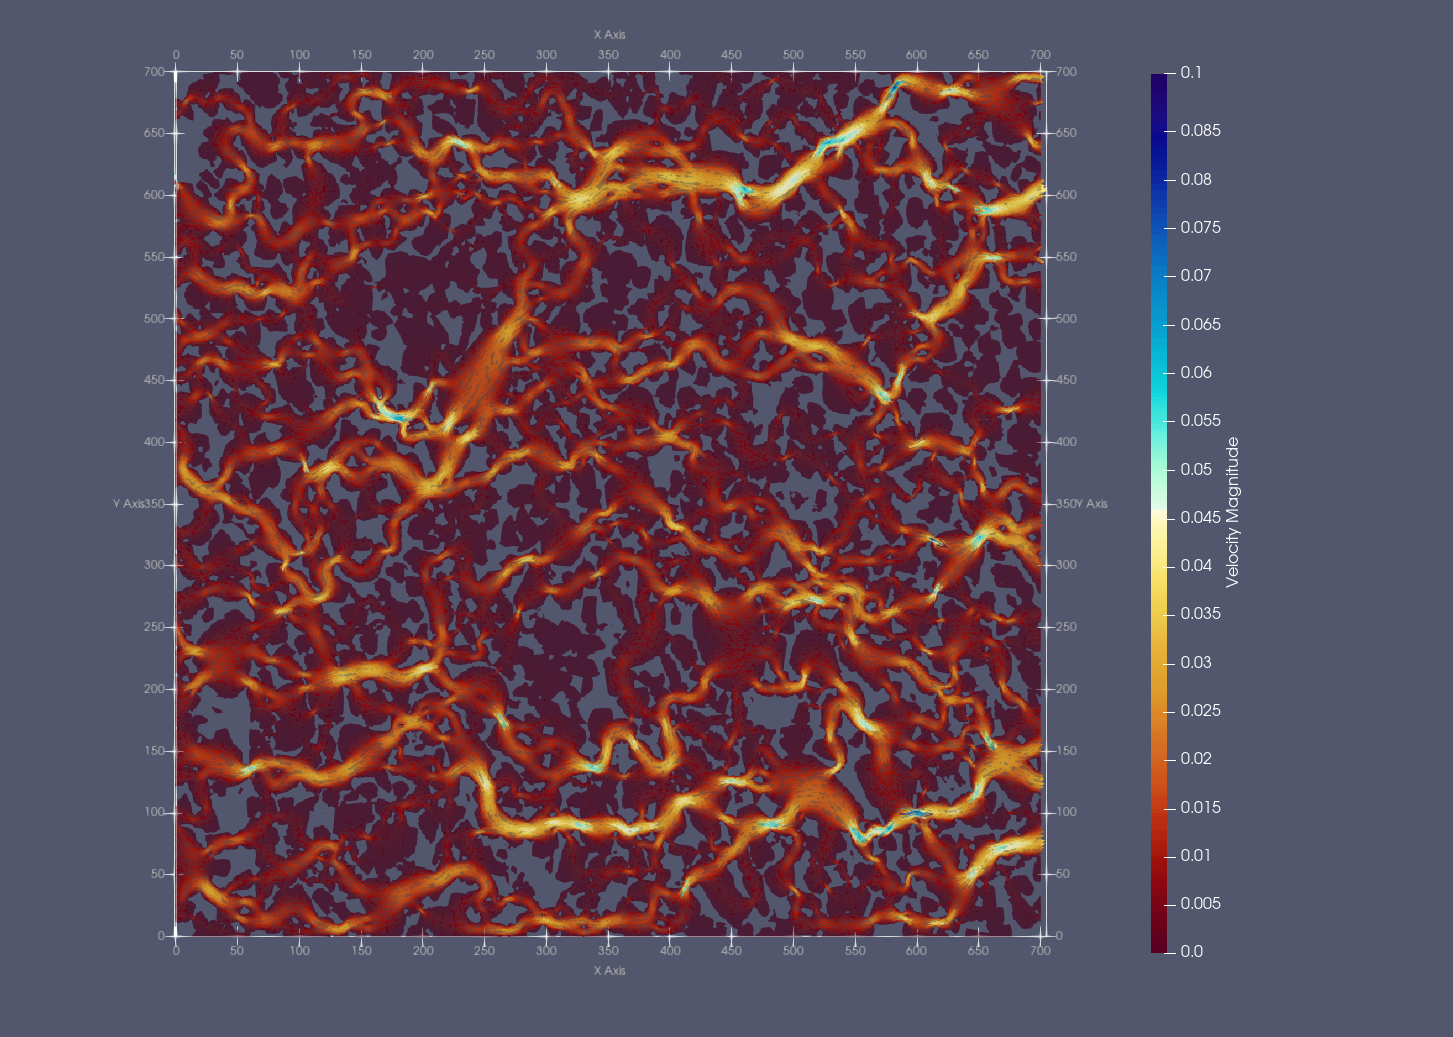
\includegraphics[width=.9\linewidth]{pics/pmVelLowV.png}
				\caption{Arbitrary porous medium (real image).}
				\label{fig:sub1}
			\end{subfigure}%
			\begin{subfigure}{.5\textwidth}
				\centering
				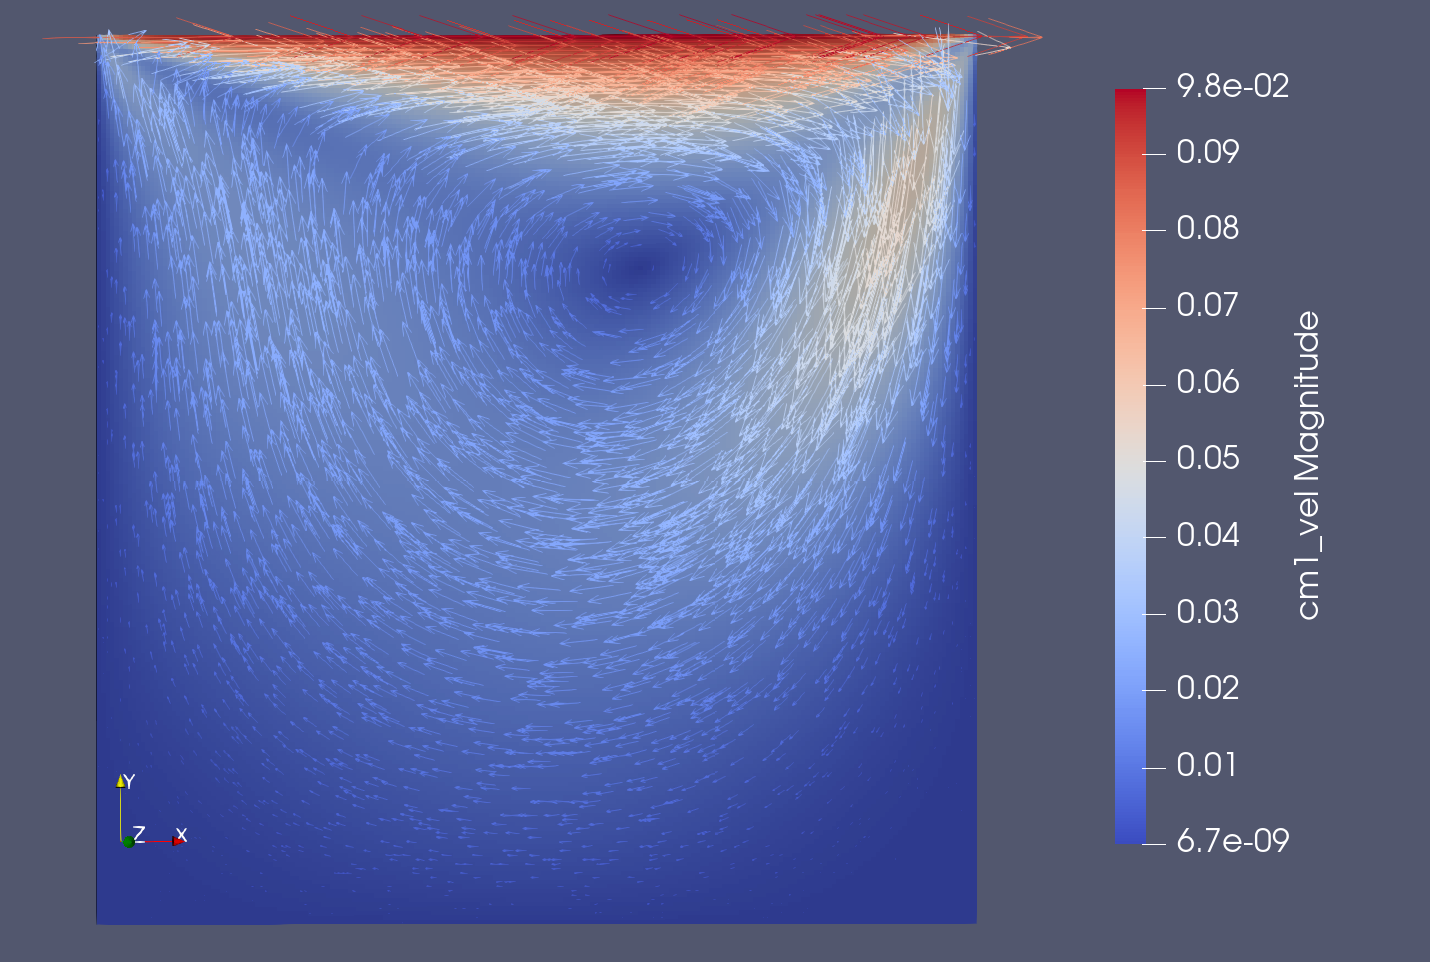
\includegraphics[width=.9\linewidth]{pics/cavity.png}
				\caption{Cavity flow, imposing a velocity on the upper wall.}
				\label{fig:sub2}
			\end{subfigure}
			\caption{Single phase cases qualitatively demonstrating the ability of modeling arbitrary porous media and arbitrary boundary conditions.}
			\label{fig:osci}
		\end{figure}
	\end{frame}

	\begin{frame}{Multiphase single component - Oscillating droplet}
		\begin{figure}[h]
			\centering
			\begin{subfigure}{.5\textwidth}
				\centering
				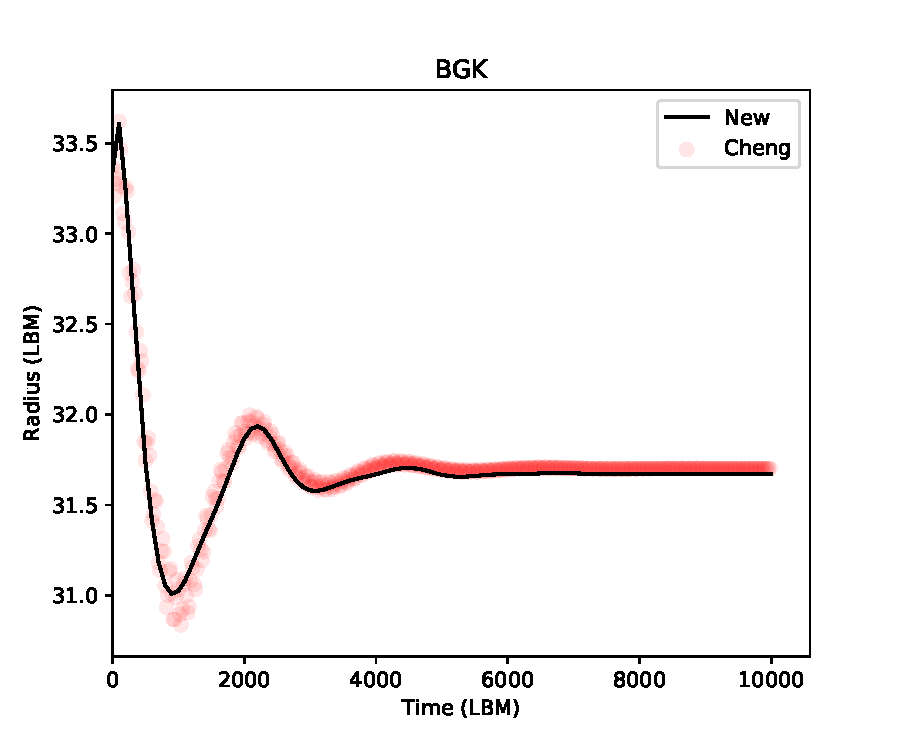
\includegraphics[width=.9\linewidth]{pics/BGKOsc.pdf}
				\caption{BGK}
				\label{fig:sub1}
			\end{subfigure}%
			\begin{subfigure}{.5\textwidth}
				\centering
				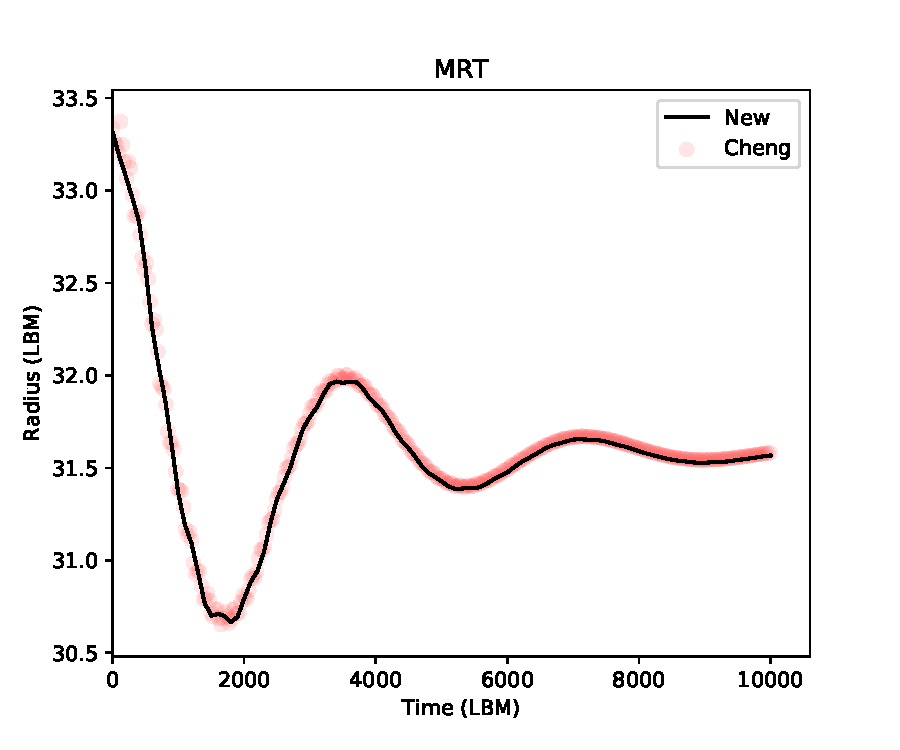
\includegraphics[width=.9\linewidth]{pics/MRTOsc.pdf}
				\caption{MRT}
				\label{fig:sub2}
			\end{subfigure}
			\caption{Oscillation droplet case. Viscosities are different in each case.}
			\label{fig:osci}
		\end{figure}
	\end{frame}
	
	\begin{frame}{Ongoing work}
		\begin{itemize}
			\item Two-component validation case
			\item Shan-Chen force in agreement with boundary conditions
			\item Viscosity per component/phase
			\item Falling and raising droplet/bubble within LBM velocity ranges (see falling droplet video).
		\end{itemize}
	\end{frame}
	
	\begin{frame}{Questions}
		\begin{itemize}
			\item<1> Mass increasing when imposing velocity/outflow.
			\begin{equation*}
			\begin{split}
				f_{i,\text{in}}^{\text{bndry}} = f_{i,\text{in}}^{\text{neighbor}} \, \, \, \text{vs.}\\
				f_{i,\text{in}}^{\text{bndry}} = f_{\bar{i},\text{in}}^{\text{bndry}} - g(\mathbf{u}_{n}^{\text{neighbor}}) \,\,\,\,\, \text{    (wall)}
			\end{split}
			\end{equation*}
			\item<1> Over-constraining P and $\mathbf{u}$ with outflow, may solve the increasing density?
			\item<2> Outflow boundary conditions. Assumptions and implications. How many layers for averaging?
			\item<2> Density variations in velocity/pressure are common in LBM?
			\item<3> Is there a general treatment for corners for all BC combinations?
			\item<3> $\Psi(P) \text{ .vs. } \Psi^i(P_i)$. Was this tried and what were the difficulties?
			\item<3> Velocity modification. Which $\tau$ to use in two-phase systems?
			\begin{equation}
			\mathbf{u}^{mod} = \mathbf{u} + \frac{\beta \mathbf{F}}{(\tau - 0.5)\psi^2}
			\end{equation}
		\end{itemize}
	\end{frame}

	\begin{frame}{Density variations}
		\begin{columns}
			\column{0.5\textwidth}
			\begin{figure}
				\centering
				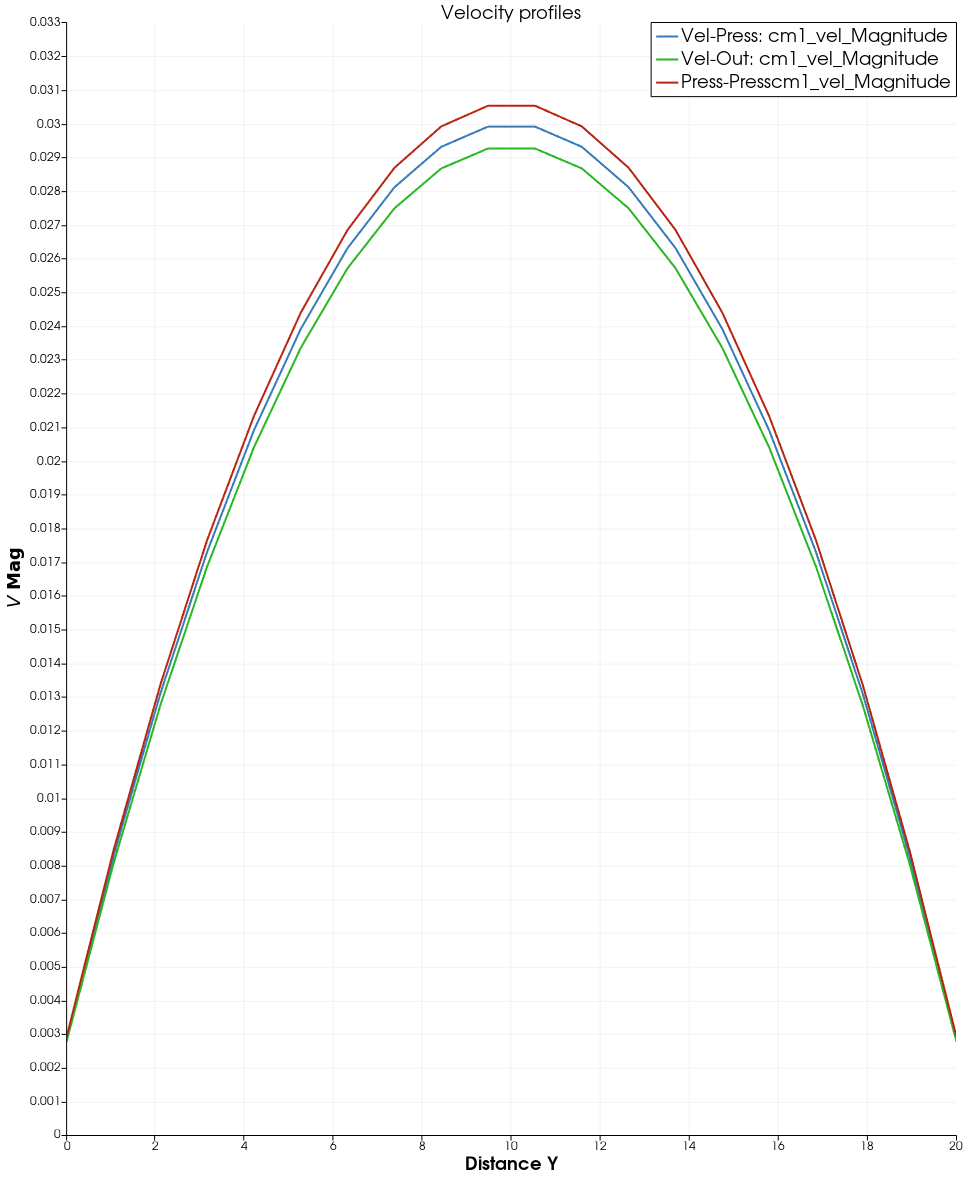
\includegraphics[width=\textwidth]{pics/velDropBox.png}
				%\caption[]{}    
				\label{}
			\end{figure}
			
			\column{0.5\textwidth}
			
			\begin{figure}
				\centering
				
				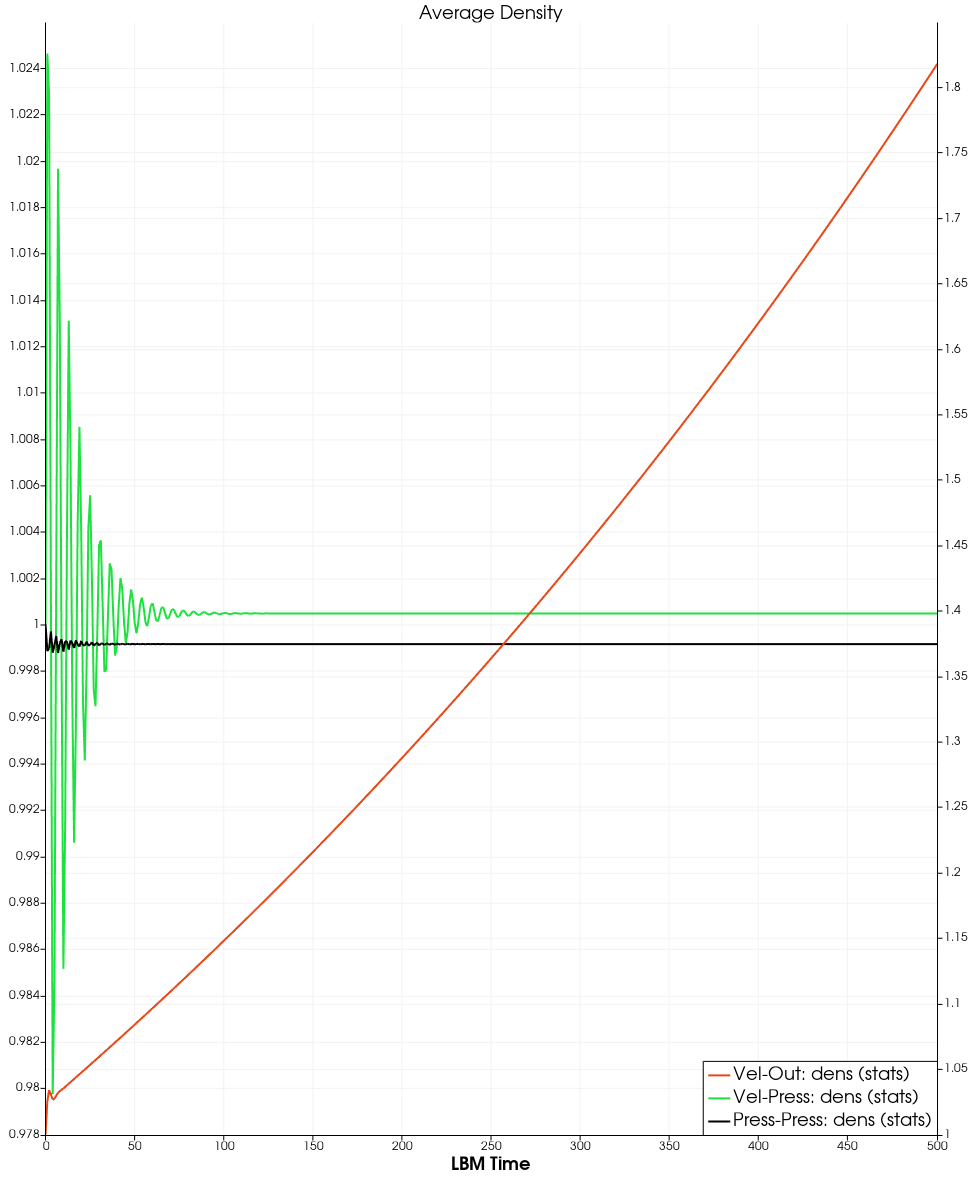
\includegraphics[width=0.8\textwidth]{pics/globalDenBox.png}
				%\caption[]{}   
				\label{}
			\end{figure}
		\end{columns}
	\end{frame}
	
	\begin{frame}{\href{https://www.overleaf.com/project/5f5cfacb13ed640001eeb63d}{\color{green}Paper}}
		
		What cases were selected for validation?\\~\\
		
		Ideas/tasks for dynamic validations:
		\begin{itemize}
			\item Young-Laplace equation
			\item Find analytical expression for oscillation frequency
			\item Rayleigh-Taylor instability (surface waves)
			\item Rising bubble/falling droplet (simple analytical solution in 3D!)
			\item Impacting droplet
		\end{itemize}
	
	Starting with the Young-Laplace case is straightforward, if this case will go in the paper.
	\end{frame}
	
	\begin{frame}{Discussion}
		Discussion...
	\end{frame}
	%---------------------------------------------------------
	%---------------------------------------------------------
	%---------------------------------------------------------
	%---------------------------------------------------------
	%---------------------------------------------------------
	%---------------------------------------------------------
	%---------------------------------------------------------
	%---------------------------------------------------------
	%---------------------------------------------------------
	
	\begin{frame}{Input}
		\begin{figure}
			\centering
			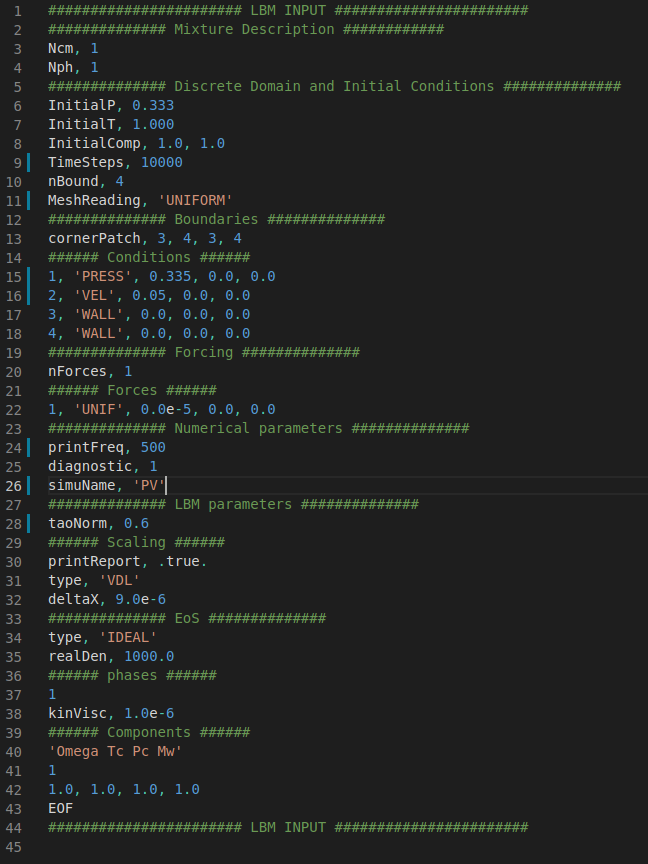
\includegraphics[width=0.5\textwidth]{pics/modelInput.png}
		\end{figure}
	\end{frame}
	
	\begin{frame}{Discussion}
		Discussion...
	\end{frame}
	
	%---------------------------------------------------------
	%---------------------------------------------------------

	\begin{frame}{template}
		\textbf{a}\\~\\
		\begin{itemize}
			\item A
			\begin{itemize}
				\item A
			\end{itemize}
		\end{itemize}
	\end{frame}
	\begin{frame}{}
		
	\end{frame}
		\begin{frame}{Discussion}
		Discussion...
	\end{frame}
	

	%---------------------------------------------------------
	\section*{Useful frame options}
	\label{}
	\justifying
	\begin{frame}
		\textbf{Report XXX XX - 202X}\\~\\
		Main discussion points:
		\begin{itemize}
			\item Topic 1
			\item Topic 2
		\end{itemize}
	\end{frame}
	%---------------------------------------------------------

	%---------------------------------------------------------
	\begin{frame}
	\end{frame}
	%---------------------------------------------------------
	%---------------------------------------------------------
	\begin{frame}
	\end{frame}
	%---------------------------------------------------------
	%---------------------------------------------------------
	\begin{frame}
	\end{frame}
	%---------------------------------------------------------
		%---------------------------------------------------------
	%Changing visivility of the text
	\begin{frame}
		\frametitle{Sample frame title}
		This is a text in second frame. For the sake of showing an example.
		
		\begin{itemize}
			\item<1-> Text visible on slide 1
			\item<2-> Text visible on slide 2
			\item<3> Text visible on slides 3
			\item<4-> Text visible on slide 4
		\end{itemize}
	\end{frame}
	
	%---------------------------------------------------------
	
	
	%---------------------------------------------------------
	%Example of the \pause command
	\begin{frame}
		In this slide \pause
		
		the text will be partially visible \pause
		
		And finally everything will be there
	\end{frame}
	%---------------------------------------------------------
	
	%---------------------------------------------------------
	%Highlighting text
	\begin{frame}
		\frametitle{Sample frame title}
		
		In this slide, some important text will be
		\alert{highlighted} because it's important.
		Please, don't abuse it.
		
		\begin{block}{Remark}
			Sample text
		\end{block}
		
		\begin{alertblock}{Important theorem}
			Sample text in red box
		\end{alertblock}
		
		\begin{examples}
			Sample text in green box. The title of the block is ``Examples".
		\end{examples}
	\end{frame}
	%---------------------------------------------------------
	
	
	%---------------------------------------------------------
	%Two columns
	\begin{frame}
		\frametitle{Two-column slide}
		
		\begin{columns}
			
			\column{0.5\textwidth}
			This is a text in first column.
			$$E=mc^2$$
			\begin{itemize}
				\item First item
				\item Second item
			\end{itemize}
			
			\column{0.5\textwidth}
			This text will be in the second column
			and on a second tought this is a nice looking
			layout in some cases.
		\end{columns}
	\end{frame}
	%---------------------------------------------------------
	
	
\end{document}